\chapter{Equações}
%\label{cap:0}

\colorbox{azul}{
 \begin{minipage}{0.9\linewidth}
 \begin{center}
   Uma equação é uma sentença matemática aberta, ou seja, sentença matemática que possui ao menos uma incógnita, e que estabelece uma igualdade entre duas expressões matemáticas.
 \end{center}
 \end{minipage}}

 \vskip0.3cm

 \begin{exem}
 A seguintes expressões matemáticas são exemplos de equações:

\begin{enumerate}[(1)]
 \item $x+1=3$;
 \item $\sin(x)=0$;
 \item $2x+3=7x-2$;
 \item $x^2+3x+1=0$;
 \item $x+y= 5$.
\end{enumerate}
\end{exem}

 E para ajudar a entender o conceito de equação, seguem algumas expressões matemáticas que não são equações, com a justificativa do porquê elas não são equações:
\begin{exem}
\begin{enumerate}[(1)]
 \item Uma desigualdade, ou seja, uma sentença matemática que relaciona duas expressões matemáticas através do sinal de diferente ($\neq$), não é uma equação, exemplo: $x+1 \neq 3$.

 \item $3 + 2 = 5$, por não ser uma sentença aberta.

 Sentenças matemáticas que relacionam duas expressões matemáticas através dos sinais de menor ($<$), maior ($>$), menor ou igual ($\leqq$), maior ou igual ($\geqq$), não são equações. Elas são chamadas de inequações. Seguem alguns exemplos:

 \item $\sin(x) < 0$, neste caso o sinal de menor $<$, nos diz que $\sin(x)$ é menor do que $0$.
 \item $2x+3 \leqq 7x-2$.
 \item $x^2+3x+1 \geqq 0$.
\end{enumerate}
\end{exem}



Vamos nos dedicar nesta seção para entender as equações de 1º grau e as de 2º grau. Mas antes vejamos um exemplo de como as equações aparecem em nosso dia-a-dia.

\begin{exem}
 Situação problema: Geraldo frequenta uma lan house, pois não tem internet em sua casa, e paga uma taxa fixa de $R\$ 1,00$ a primeira hora, mais $R\$ 2,00$ a cada hora excedente. Se após o uso Geraldo pagou $R\$ 7,00$, por quanto tempo ele usou a internet?

 \underline{Resolução:}

 Podemos concluir que Geraldo usou o computador por $4$ horas, já que pagou $R\$ 1,00$ pela primeira hora, e consequentemente $(7,00 - 1,00 = 6,00)$ $R\$ 6,00$ pelas demais horas, como cada hora a mais custa $R\$ 2,00$ e $(6,00 \div 2,00 = 3)$ temos então que Geraldo usou $(1 + 3 = 4)$ horas.

 Podemos generalizar esta situação usando a letra $x$ para representar o tempo de internet utilizado, que é o valor que não conhecemos, chegando à seguinte equação: $2x + 1 = 7$.
\end{exem}

A equação resultante desta situação problema é o que chamamos de equação do 1º grau.

\section{Equações do 1º grau}

\colorbox{azul}{
 \begin{minipage}{0.9\linewidth}
 \begin{center}
   As equações de 1º grau tem a seguinte forma geral:
 \[ax + b = 0\]
onde $a, b \in \mathbb{R}$ são números dados (conhecidos), com $a \neq 0 $.
 \end{center}
 \end{minipage}}

 \vskip0.3cm

Como resolver uma equação destas, ou equivalentemente, como encontrar o valor de $x$:
\[ax + b = 0 \Rightarrow ax= -b \Rightarrow x = \frac{-b}{a} .\]


\begin{exem}
 Como resolver equações do 1º grau:
 \begin{itemize}
  \item $2x + 4 = 0 \Rightarrow 2x = -4 \Rightarrow x = \frac{-4}{2} \Rightarrow x = -2$
  \item $3x - 5 = 4 \Rightarrow 3x = 4 +5 \Rightarrow 3x = 9 \Rightarrow x = \frac{9}{3} \Rightarrow x = 3$
  \item $3(x + 2)= 12 \Rightarrow 3x + 6 = 12 \Rightarrow 3x = 12 - 6 \Rightarrow 3x = 6 \Rightarrow x = \frac{6}{3} \Rightarrow x = 2 $
  \item $ax = 0$

  Neste caso $a \neq 0$, como produto de dois números só é zero quando um deles for igual a zero concluímos que $x = 0$.
  \end{itemize}
\end{exem}

\newpage
\section{Equações do 2º grau}

\colorbox{azul}{
 \begin{minipage}{0.9\linewidth}
 \begin{center}
   As equações de 2º grau tem a seguinte forma geral:
   \[ax^2 + bx + c = 0\]
  onde $a, b, c \in \mathbb{R}$ são números dados (conhecidos), com $a \neq 0 $.
 \end{center}
 \end{minipage}}

 \vskip0.3cm

Para resolver este tipo de equação usamos a fórmula da equação do 2º grau também conhecida como a fórmula de Bhaskara, dada por:

 \vskip0.3cm
 \begin{center}
 \textbf{Fórmula de Bhaskara}
   \[\destaque{x= \frac{-b \pm \sqrt{b^2 - 4ac}}{2a}}\]
 \end{center}

Lembremos que $z^2= (-z)^2$ e que extrair a raiz quadrada de um número $y$ é procurar o número $z$ tal que $z= -\sqrt{y}$ e $z= \sqrt{y}$ donde obtemos que $z= \pm \sqrt{y}$. Por isso precisamos colocar o sinal $(\pm)$ antes da raiz quadrada na equação acima.

A fórmula de Bhaskara é também reescrita da seguinte forma:
\[\destaque{x= \frac{-b \pm \sqrt{\Delta}}{2a}} \ \ \ \text{ para } \ \ \ \destaque{\Delta= b^2 - 4ac}\]
a partir da análise do sinal de delta determinamos se as equações do 2º grau possuem $0$, $1$ ou $2$ soluções diferentes no conjunto dos números reais, da seguinte forma:
\begin{itemize}
\item Se $\Delta < 0$ a equação não possui raízes reais, pois em $\R$ não existe raíz quadrada de número negativo.
\item Se $\Delta = 0$ a equação possui apenas a solução $x= \frac{-b}{2a}$.
\item Se $\Delta > 0$ a equação possui duas raízes reais diferentes, $x_1= \frac{-b - \sqrt{\Delta}}{2a}$ e $x_2= \frac{-b + \sqrt{\Delta}}{2a}$.
\end{itemize}


Antes de usar esta fórmula especificamente para resolver as equações do 2º grau vejamos alguns casos particulares de equações do 2º grau que podemos resolver sem esta fórmula.

 \subsection{Caso \texorpdfstring{$b=0$}{b=0}}

 Neste caso a equação é da forma:
 \[ax^2 + 0x + c= 0 \Rightarrow ax^2 + c= 0\]
 note que neste caso podemos facilmente isolar o $x^2$, e então fica fácil de resolver a equação, veja o passo a passo da resolução:
 \[ax^2 + c= 0 \Rightarrow ax^2= -c \Rightarrow x^2= \frac{-c}{a} \Rightarrow x= \pm \sqrt{\frac{-c}{a}}\]

 \begin{exem} Vejamos alguns exemplos de equações deste tipo resolvidas.
 \begin{enumerate}[1)]
 \item Resolva a equação $2x^2 - 32=0$
 \[2x^2 - 32=0 \Rightarrow 2x^2= 32 \Rightarrow x^2= \frac{32}{2} \Rightarrow x= \pm \sqrt{16} \Rightarrow x= \pm 4 \ .\]
 Logo $x= -4$ e $x= 4$ são soluções desta equação. Então o conjunto solução desta equação é $S= \{-4, 4\}$.

 \item Resolva a equação $2x^2 - 36=0$

 \[2x^2 - 36=0 \Rightarrow 2x^2= 36 \Rightarrow x^2= \frac{36}{2} \]
 a partir daqui podemos dar continuidade a resolução desta equação de duas formas diferentes, segue abaixo as duas formas para que você possa comparar e escolher um caminho para seguir,
 \begin{eqnarray*}
 \Rightarrow
 \begin{cases}
 x^2= \dfrac{36}{2} \Rightarrow x^2= 18 \Rightarrow x= \pm \sqrt{18}= \pm \sqrt{2 \cdot 3^2}= \pm 3\sqrt{2} \\
 x^2= \dfrac{36}{2} \Rightarrow x= \pm \sqrt{\dfrac{36}{2}} \Rightarrow x= \pm \dfrac{\sqrt{36}}{\sqrt{2}} \Rightarrow x= \pm \dfrac{6}{\sqrt{2}} \cdot \dfrac{\sqrt{2}}{\sqrt{2}} \Rightarrow x= \pm  \dfrac{6\sqrt{2}}{2}= \pm 3\sqrt{2} \ .
 \end{cases}
 \end{eqnarray*}
 Portanto o conjunto solução desta equação é $S= \left\{-3\sqrt{2}, 3\sqrt{2}\right\}$.

  \item Resolva a equação $x^2 - 81=0$
 \[x^2 - 81=0 \Rightarrow x^2= 81 \Rightarrow x^2= \frac{81}{1} \Rightarrow x= \pm \sqrt{81} \Rightarrow x= \pm 9 \ .\]
 Logo $x= -9$ e $x= 9$ são soluções desta equação. Então o conjunto solução desta equação é $S= \{-9, 9\}$.

  \item Resolva a equação $x^2 + 256=0$
 \[x^2 +256=0 \Rightarrow x^2= -256 \Rightarrow x^2= \frac{-256}{1} \Rightarrow x= \pm \sqrt{-256} \ .\]
 Como no conjunto dos números reais não existe raíz quadrada de número negativo, decorre que não existe $\sqrt{-256}$ no conjunto dos números reais, logo esta equação não tem solução no conjunto dos números reais.

   \item Resolva a equação $-2x^2 + 8=0$
 \[-2x^2 + 8=0 \Rightarrow -2x^2= -8 \Rightarrow x^2= \frac{-8}{-2} \Rightarrow x= \pm \sqrt{4} \Rightarrow x= \pm 2 \ .\]
 Logo $x= -2$ e $x= 2$ são soluções desta equação. Então o conjunto solução desta equação é $S= \{-2, 2\}$.

   \item Resolva a equação $\dfrac{32}{6}x^2 - \dfrac{100}{12}=0$
   \begin{eqnarray*}
   \dfrac{32}{6}x^2 - \dfrac{100}{12} &=& 0 \\
   \dfrac{32}{6}x^2 &=& \dfrac{100}{12} \\
   x^2 &=& \dfrac{100}{12} \cdot \dfrac{6}{32} \\
   x^2 &=& \dfrac{100}{2} \cdot \dfrac{1}{32} = \dfrac{100}{64} \\
   x &=& \pm \sqrt{\dfrac{100}{64}} = \pm \dfrac{10}{8} = \pm \dfrac{5}{4} \ .
   \end{eqnarray*}


 Então o conjunto solução desta equação é $S= \left\{-\dfrac{5}{4}, \dfrac{5}{4} \right\}$.
 \end{enumerate}
 \end{exem}

 \begin{exer}
 Resolva as seguintes equações do 2º grau:

 \begin{multicols}{3}
 \begin{enumerate}[a)]
 \item $x^2 - 36=0$
 \item $x^2 - 169=0$
 \item $x^2 - 225=0$
 \item $x^2 - 16=0$
 \item $x^2 - 121=0$
 \item $x^2 - 8=0$
 \item $x^2 - 27=0$
 \item $x^2 - 125=0$
 \item $9x^2 - 4=0$
 \item $25x^2 - 49=0$
 \item $81x^2 - 64=0$
 \item $x^2 + 4=0$
 \item $x^2 + 25=0$
 \item $3x^2 + 300=0$
 \item $3x^2 - 75=0$
 \item $-2x^2 + 18=0$
 \item $-3x^2 + 108=0$
 \item $-x^2 + 225=0$
 \item $\dfrac{3}{2}x^2 - \dfrac{27}{8}= 0$
 \item $\dfrac{81}{6}x^2 - \dfrac{100}{6}= 0$
 \end{enumerate}
 \end{multicols}
 \end{exer}

 \subsection{Caso \texorpdfstring{$c=0$}{c=0}}

 Neste caso a equação é da forma:
 \[ax^2 + bx + 0= 0 \Rightarrow ax^2 + bx= 0\]
 note que neste caso podemos facilmente isolar o $x$, e então fica fácil de resolver a equação, veja o passo a passo da resolução:
 \[ax^2 + bx= 0 \Rightarrow x \cdot (ax + b)= 0 \Rightarrow
 \begin{cases}
 x_1= 0 \\
 ax+b=0 \Rightarrow ax= -b \Rightarrow x_2= \dfrac{-b}{a} \ .
 \end{cases}
  \]

 Portanto as soluções desta equação são $x= 0$ e $x= \dfrac{-b}{a}$.

 \begin{exem} Vejamos alguns exemplos numéricos de equações deste tipo resolvidas.
 \begin{enumerate}[1)]
 \item Resolva a equação $x^2 + 40x=0$
 \[x^2 + 40x=0 \Rightarrow x \cdot (x+ 40)= 0 \Rightarrow
 \begin{cases}
 x_1=0 \\
 x+40=0 \Rightarrow x_2= -40 \ .
 \end{cases}
 \]
 Portanto as soluções desta equação são $x_1= 0$ e $x_2= -40$. O conjunto solução desta equação é $S= \left\{ -40, 0 \right\}$.

 \item Resolva a equação $x^2 + \sqrt[3]{5}x=0$
 \[x^2 + \sqrt[3]{5}x=0 \Rightarrow x \cdot (x+ \sqrt[3]{5})= 0 \Rightarrow
 \begin{cases}
 x_1=0 \\
 x+\sqrt[3]{5}=0 \Rightarrow x_2= -\sqrt[3]{5} \ .
 \end{cases}
 \]
 Portanto as soluções desta equação são $x_1= 0$ e $x_2= -\sqrt[3]{5}$. O conjunto solução desta equação é $S= \left\{ -\sqrt[3]{5}, 0 \right\}$.

 \item Resolva a equação $7x^2 - \sqrt{98}x=0$
\begin{align*}
7x^2 - \sqrt{98}x=0
& \Rightarrow x \cdot (7x - \sqrt{98})= 0 \\
& \Rightarrow
 \begin{cases}
 x_1=0 \\
 7x - \sqrt{98}=0
\Rightarrow 7x = \sqrt{7^2 \cdot 2}
\Rightarrow x= \frac{7\sqrt{2}}{7}
\Rightarrow x_2= \sqrt{2} \ .
 \end{cases}
\end{align*} 
 
% \[ \]
 Portanto as soluções desta equação são $x_1= 0$ e $x_2= \sqrt{2}$. O conjunto solução desta equação é $S= \left\{ \sqrt{2}, 0 \right\}$.

 \item Resolva a equação $\dfrac{3}{2}x^2 + \dfrac{3}{2}x=0$

 \[\dfrac{3}{2}x^2 + \dfrac{3}{2}x=0 \Rightarrow x \cdot (\dfrac{3}{2}x+ \dfrac{3}{2})= 0 \]

 \[\Rightarrow
 \begin{cases}
 x_1=0 \\
 \dfrac{3}{2}x + \dfrac{3}{2}=0 \Rightarrow \dfrac{3}{2}x= -\dfrac{3}{2} \Rightarrow x= -\dfrac{3}{2} \div \dfrac{3}{2} \Rightarrow x= -\dfrac{3}{2} \cdot \dfrac{2}{3} \Rightarrow x_2= -1 \ .
 \end{cases} \]

 Portanto as soluções desta equação são $x_1= 0$ e $x_2= -1$. O conjunto solução desta equação é $S= \left\{ -1, 0 \right\}$.

 \item Resolva a equação $\sqrt{2}x^2 - \sqrt{50}x=0$
 \[\sqrt{2}x^2 - \sqrt{50}x=0 \Rightarrow x \cdot (\sqrt{2}x - \sqrt{50})= 0 \]
 \[\Rightarrow
 \begin{cases}
 x_1=0 \\
 \sqrt{2}x - \sqrt{50}=0 \Rightarrow x= \frac{\sqrt{50}}{\sqrt{2}} \Rightarrow x= \sqrt{\dfrac{50}{2}} \Rightarrow x= \sqrt{25} \Rightarrow x_2= 5 \ .
 \end{cases}
 \]
 Portanto as soluções desta equação são $x_1= 0$ e $x_2= 5$. O conjunto solução desta equação é $S= \left\{ 0, 5 \right\}$.
 \end{enumerate}
 \end{exem}

 \begin{exer} Resolva as seguintes equações do 2º grau:
 \begin{multicols}{3}
 \begin{enumerate}[a)]
 \item $x^2 - 36x=0$
 \item $x^2 - 13x=0$
 \item $x^2 - \sqrt{2}x=0$
 \item $x^2 + 13x=0$
 \item $x^2 + 17x=0$
 \item $x^2 - 23x=0$
 \item $2x^2 - 2\sqrt{3}x= 0$
 \item $3x^2 + 15x=0$
 \item $-4x^2 + 24x=0$
 \item $\dfrac{1}{3}x^2 - 37x=0$
 \item $\dfrac{3}{5}x^2 - \dfrac{3}{20}x=0$
 \item $\sqrt{5}x^2 - \sqrt{180}x=0$
 \item $\dfrac{2}{3}x^2 - \dfrac{2}{3}x=0$
 \item $5x^2 + \sqrt{50}x= 0$
 \end{enumerate}
 \end{multicols}
 \end{exer}

 \subsection{Caso \texorpdfstring{$b=c=0$ e $a \neq 0$}{b=c=0 e a não nulo}}

 Neste caso as equações do 2º grau são do tipo
 \[ax^2 = 0 \ . \]

  Notemos que o produto de dois números só é zero quando um deles for igual a zero, donde concluímos que $x^2 = 0 \Rightarrow x =0$. Portanto o conjunto solução deste tipo de equação, independente do valor de $a$ é $S= \left\{ 0 \right\}$.

  \begin{exem} Considerando a equação $23x^2=0$ temos,
  \[23x^2= 0 \Rightarrow x^2=0 \Rightarrow x= 0 \ , \]
  logo neste caso o conjunto solução é $S= \left\{ 0 \right\}$.
  \end{exem}

 \subsection{Equação completa \texorpdfstring{$ax^2+ bx + c = 0$}{ax² + bx + c = 0}}
  
 Neste caso temos $a \neq 0$, $b \neq 0$ e $c \neq 0$, então para resolver a equação de forma geral dada por: 
 \[ax^2+ bx + c = 0 \]
 precisamos utilizar a fórmula
 \[x = \dfrac{-b \pm \sqrt{b^2 - 4 \cdot a \cdot c}}{2 \cdot a} \ ,\]
 conhecida como fórmula da equação do 2º grau ou fórmula de Báskara.


 \begin{exem} Vejamos alguns exemplos de como resolver este tipo de equação.
 \begin{enumerate}[1)]
 \item Resolva a equação $x^2 + 4x + 4= 0$.

 Como esta equação tem os valores de $a, b, c$ diferentes de zero, precisamos obrigatóriamente utilizar a fórmula da equação do 2º grau para resolver. Note que neste caso temos:
  \begin{itemize}
  \item $a= 1$, que é o valor que multiplica o $x^2$;
  \item $b= 4$, que é o valor que multiplica o $x$;
  \item $c= 4$, que é o termo independente da equação.
  \end{itemize}
  Assim substituindo na fórmula

 \[x = \dfrac{-b \pm \sqrt{b^2 - 4 \cdot a \cdot c}}{2 \cdot a} \ ,\]
 obtemos:

 \begin{eqnarray*}
 x &=& \dfrac{-4 \pm \sqrt{4^2 - 4 \cdot 1 \cdot 4}}{2 \cdot 1} \\
 x &=& \dfrac{-4 \pm \sqrt{16 - 16}}{2}= \dfrac{-4 \pm \sqrt{0}}{2}= \dfrac{-4 \pm 0}{2} \\
 x &=& \dfrac{-4}{2}= -2
 \end{eqnarray*}

 Portanto esta equação possui $x= -2$ como solução. Logo o conjunto solução é $S= \{-2\}$.

 \item Resolva a equação $x^2 - 10x + 25= 0$.

 Note que neste caso temos:
  \begin{itemize}
  \item $a= 1$, que é o valor que multiplica o $x^2$;
  \item $b= -10$, que é o valor que multiplica o $x$;
  \item $c= 25$, que é o termo independente da equação.
  \end{itemize}
  Assim substituindo na fórmula

 \[x = \dfrac{-b \pm \sqrt{b^2 - 4 \cdot a \cdot c}}{2 \cdot a} \ ,\]
 obtemos:

 \begin{eqnarray*}
 x &=& \dfrac{-(-10) \pm \sqrt{(-10)^2 - 4 \cdot 1 \cdot 25}}{2 \cdot 1} \\
 x &=& \dfrac{10 \pm \sqrt{100 - 100}}{2}= \dfrac{10 \pm \sqrt{0}}{2}= \dfrac{10 \pm 0}{2} \\
 x &=& \dfrac{10}{2}= 5
 \end{eqnarray*}

 Portanto esta equação possui $x= 5$ como solução.  Logo o conjunto solução é $S= \{5\}$.

 \item Resolva a equação $x^2+2x-15= 0$.

 Note que neste caso temos:
  \begin{itemize}
  \item $a= 1$, que é o valor que multiplica o $x^2$;
  \item $b= 2$, que é o valor que multiplica o $x$;
  \item $c= -15$, que é o termo independente da equação.
  \end{itemize}
  Assim substituindo na fórmula

 \[x = \dfrac{-b \pm \sqrt{b^2 - 4 \cdot a \cdot c}}{2 \cdot a} \ ,\]
 obtemos:

 \begin{eqnarray*}
 x &=& \dfrac{-2 \pm \sqrt{2^2 - 4 \cdot 1 \cdot (-15)}}{2 \cdot 1} \\
 x &=& \dfrac{-2 \pm \sqrt{4 + 60}}{2}= \dfrac{-2 \pm \sqrt{64}}{2}= \dfrac{-2 \pm 8}{2} \\
 x_1 &=& \dfrac{-2 + 8}{2}= \dfrac{6}{2}= 3 \\
 x_2 &=& \dfrac{-2 - 8}{2}= \dfrac{-10}{2}= -5
 \end{eqnarray*}

 Portanto esta equação possui $x_1= 3$ e $x_2= -5$ como solução. Logo o conjunto solução é $S= \{-5, 3\}$.

  \item Resolva a equação $2x^2 - 5x - 3= 0$.

 Note que neste caso temos:
  \begin{itemize}
  \item $a= 2$;
  \item $b= -5$;
  \item $c= -3$.
  \end{itemize}
  Assim substituindo na fórmula

 \[x = \dfrac{-b \pm \sqrt{b^2 - 4 \cdot a \cdot c}}{2 \cdot a} \ ,\]
 obtemos:

 \begin{eqnarray*}
 x &=& \dfrac{-(-5) \pm \sqrt{(-5)^2 - 4 \cdot 2 \cdot (-3)}}{2 \cdot 2} \\
 x &=& \dfrac{5 \pm \sqrt{25 + 24}}{4}= \dfrac{5 \pm \sqrt{49}}{4}= \dfrac{5 \pm 7}{4} \\
 x_1 &=& \dfrac{5 + 7}{4}= \dfrac{12}{4}= 3 \\
 x_2 &=& \dfrac{5 - 7}{4}= \dfrac{-2}{4}= \dfrac{-1}{2}
 \end{eqnarray*}

 Portanto esta equação possui $x_1= 3$ e $x_2= \dfrac{-1}{2}$ como solução. Logo o conjunto solução é $S= \left\{3, \dfrac{-1}{2}\right\}$.

  \item Resolva a equação $-8x^2 - 2x + 3= 0$.

 Note que neste caso temos:
  \begin{itemize}
  \item $a= -8$;
  \item $b= -2$;
  \item $c= 3$.
  \end{itemize}
  Assim substituindo na fórmula

 \[x = \dfrac{-b \pm \sqrt{b^2 - 4 \cdot a \cdot c}}{2 \cdot a} \ ,\]
 obtemos:

 \begin{eqnarray*}
 x &=& \dfrac{-(-2) \pm \sqrt{(-2)^2 - 4 \cdot (-8) \cdot (3)}}{2 \cdot (-8)} \\
 x &=& \dfrac{2 \pm \sqrt{4 + 96}}{-16}= \dfrac{2 \pm \sqrt{100}}{-16}= \dfrac{2 \pm 10}{-16} \\
 x_1 &=& \dfrac{2 + 10}{-16}= \dfrac{12}{-16}= \dfrac{-6}{8}= \dfrac{-3}{4} \\
 x_2 &=& \dfrac{2 - 10}{-16}= \dfrac{-8}{-16}= \dfrac{4}{8}= \dfrac{1}{2}
 \end{eqnarray*}

 Logo o conjunto solução é $S= \left\{ \dfrac{-3}{4}, \dfrac{1}{2} \right\}$.

 \item Número áureo ou Número de ouro. Resolva a equação $x^2 - x - 1= 0$.

 Note que neste caso temos:
  \begin{itemize}
  \item $a= 1$;
  \item $b= -1$;
  \item $c= -1$.
  \end{itemize}
  Assim substituindo na fórmula

 \[x = \dfrac{-b \pm \sqrt{b^2 - 4 \cdot a \cdot c}}{2 \cdot a} \ ,\]
 obtemos:

 \begin{eqnarray*}
 x &=& \dfrac{-(-1) \pm \sqrt{(-1)^2 - 4 \cdot (1) \cdot (-1)}}{2 \cdot (1)} \\
 x &=& \dfrac{1 \pm \sqrt{1 + 4}}{2}= \dfrac{1 \pm \sqrt{5}}{2} \\
 x_1 &=& \dfrac{1 + \sqrt{5}}{2} \\
 x_2 &=& \dfrac{1 - \sqrt{5}}{2}
 \end{eqnarray*}

 Logo o conjunto solução é $S= \left\{ \dfrac{1 - \sqrt{5}}{2}, \dfrac{1 + \sqrt{5}}{2} \right\}$.

  \item Resolva a equação $x^2 - 2 \pi x - 4= 0$.

 Note que neste caso temos:
  \begin{itemize}
  \item $a= 1$;
  \item $b= -2 \pi $ ;
  \item $c= -4$ .
  \end{itemize}
  Assim substituindo na fórmula

 \[x = \dfrac{-b \pm \sqrt{b^2 - 4 \cdot a \cdot c}}{2 \cdot a} \ ,\]
 obtemos:
 \begin{eqnarray*}
 x &=& \dfrac{-(-2\pi) \pm \sqrt{(-2\pi)^2 - 4 \cdot 1 \cdot (-4)}}{2 \cdot 1} \\
 x &=& \dfrac{ 2 \pi \pm \sqrt{ 4 \pi^2 + 16}}{2} \\
 x &=& \dfrac{ 2 \pi \pm \sqrt{ 4 (\pi^2 + 4)}}{2} \\
 x &=& \dfrac{ 2 \pi \pm 2 \cdot \sqrt{ \pi^2 + 4}}{2} \\
 x &=& \pi \pm \sqrt{\pi^2 + 4} \\
 \end{eqnarray*}

 Portanto, $S= \left\{ \pi - \sqrt{\pi^2 + 4}, \pi + \sqrt{\pi^2 + 4} \right\}$.

 \item Resolva a equação $99x^2 - 2000x + 10000= 0$.

 Note que neste caso temos:
  \begin{itemize}
  \item $a= 99$;
  \item $b= -2000= -2 \times 10^3$ ;
  \item $c= 10000= 1 \times 10^4$ .
  \end{itemize}
  Assim substituindo na fórmula

 \[x = \dfrac{-b \pm \sqrt{b^2 - 4 \cdot a \cdot c}}{2 \cdot a} \ ,\]
 obtemos:

 \begin{eqnarray*}
 x &=& \dfrac{-(-2000) \pm \sqrt{(-2 \cdot 10^3)^2 - 4 \cdot (99) \cdot (1 \cdot 10^4)}}{2 \cdot (99)} \\
 x &=& \dfrac{ 2000 \pm \sqrt{(-2)^2 \cdot (10^3)^2 - 396 \cdot 10^4}}{198} \\
 x &=& \dfrac{ 2000 \pm \sqrt{4 \cdot 10^6 - 396 \cdot 10^4}}{198} \\
 x &=& \dfrac{ 2000 \pm \sqrt{4 \cdot 10^2 \cdot 10^4 - 396 \cdot 10^4}}{198} \\
 x &=& \dfrac{ 2000 \pm \sqrt{400 \cdot 10^4 - 396 \cdot 10^4}}{198} \\
 x &=& \dfrac{ 2000 \pm \sqrt{4 \cdot 10^4}}{198} \\
 x &=& \dfrac{ 2000 \pm \sqrt{4} \cdot \sqrt{10^4}}{198} \\
 x &=& \dfrac{ 2000 \pm 2 \cdot 10^2}{198} \\
 x &=& \dfrac{ 2000 \pm 200}{198} \\
 x_1 &=& \dfrac{ 2000 + 200}{198} = \dfrac{2200}{198} = \dfrac{100}{9} \\
 x_2 &=& \dfrac{ 2000 - 200}{198} = \dfrac{1800}{198} = \dfrac{100}{11}
 \end{eqnarray*}

 Logo o conjunto solução é $S= \left\{ \dfrac{100}{9}, \dfrac{100}{11} \right\}$.

 \end{enumerate}
 \end{exem}

 \begin{exer} Resolva as seguintes equações do 2º grau completas.
 \begin{multicols}{2}
 \begin{enumerate}[a)]
 \item $x^2 + 8x + 16=0$
 \item $x^2 - 14x + 49=0$
 \item $x^2 - 2x - 35=0$
 \item $x^2 + 3x - 18=0$
 \item $4x^2 - 27x - 7=0$
 \item $x^2 + x + \dfrac{6}{25}$
 \item $2x^2 - 2x - 2=0$
 \item $2x^2 - 2x - 5=0$
 \item $x^2 + 2x - 1=0$
 \item $91x^2 + 600x - 10000=0$
 \item $221x^2 + 3000x - 10000=0$
 \end{enumerate}
 \end{multicols}
 \end{exer}

\vskip0.3cm

\begin{exem} Todas as equações do 2º grau incompletas podem também ser resolvidas utilizando a fórmula da equação do 2º grau. Vamos dar agora dois exemplos em que as equações estão sendo resolvidas das duas formas possíveis para que você possa comparar as diferenças entre as resoluções.

 \begin{enumerate}[I)]

  \item Equação do 2º grau incompleta do tipo $c=0$ ou $ax^2 + bx = 0$:
  \[x^2 - 3x = 0\]
  1ª forma:

  $a = 1$, $b = -3$ e $c = 0$ assim usando a fórmula chegamos:
  \[x = \frac{- (-3) \pm \sqrt{(-3)^2 - 4 (1)(0)}}{2 (1)}\]
  \[\Rightarrow x = \frac{3 \pm \sqrt{9}}{2} \Rightarrow \begin{cases}
                                                          x' = \frac{3 + 3}{2} \Rightarrow x' = \frac{6}{2} \Rightarrow x' = 3 \\
                                                          x'' = \frac{3 - 3}{2} \Rightarrow x''= \frac{0}{2} \Rightarrow x''= 0
                                                         \end{cases}\]

  2ª forma:
  \[x^2 - 3x = 0 \Rightarrow x(x - 3)=0 \Rightarrow \begin{cases}
                                                     x''= 0 \\
                                                     x - 3 = 0 \Rightarrow x' = 3
                                                    \end{cases}\]


  \item Equação do 2º grau incompleta do tipo $b=0$ ou $ax^2 + c = 0$:
  \[2x^2 - 128 = 0\]
  1ª forma:

  $a = 2$, $b = 0$ e $c = -128$ assim usando a fórmula chegamos:
  \[x = \frac{- (0) \pm \sqrt{(0)^2 - 4 (2)(-128)}}{2 (2)}\]
  \[\Rightarrow x = \frac{0 \pm \sqrt{1024}}{4} \Rightarrow \begin{cases}
                                                          x' = \frac{ 0 + 32}{4} \Rightarrow x' = \frac{32}{4} \Rightarrow x' = 8 \\
                                                          x'' = \frac{0 - 32}{4} \Rightarrow x''= \frac{-32}{4} \Rightarrow x''= -8
                                                         \end{cases}\]


  2ª forma:
  \[2x^2 - 128 = 0 \Rightarrow 2x^2 = 128 \Rightarrow x^2 = \frac{128}{2} \Rightarrow x^2 = 64 \Rightarrow x = \pm \sqrt{64} \Rightarrow x = \pm 8 \ .\]
  \end{enumerate}
\end{exem}

\subsection{Caso \texorpdfstring{$(x+a)\cdot (x+b)= 0$}{(x+a)(x+b) = 0}}
 Neste caso vamos considerar as equações do tipo
\[(x+a)\cdot (x+b)= 0\]
para $a, b \in \R$ quaisquer.

Para resolver equações dadas desta forma um dos caminhos é lembrar que,
\[(x+a)\cdot (x+b)= x^2 + bx + ax + ab= x^2 + (a + b)x + ab\]
fazendo isso obtemos a equação do 2º grau $x^2 + (a + b)x + ab= 0$ na qual aplicamos a fórmula de Bhaskara.

Outra forma de resolver equações dadas desta forma, é lembrar que $\forall u, v \in \R$ temos que
\[u \cdot v= 0 \Leftrightarrow u= 0 \ \ \ \text{ ou } \ \ \ v=0 \ .\]
Considerando portanto $u= x+a$ e $v= x+b$ com $a, b \in \R$ dados, obtemos que
\[u \cdot v= (x+a)\cdot (x+b)= 0 \Leftrightarrow x+a= 0 \ \ \ \text{ ou } \ \ \ x+b=0\]
assim a resolução deste tipo de equação do 2º grau se torna a resolução de duas equações do 1º grau.

\begin{exem}
\begin{enumerate}[1)]
\item Resolva a equação $(x - \pi) \cdot (x - e)= 0$.
\[(x - \pi) \cdot (x - e)= 0 \Rightarrow
\begin{cases}
 x - \pi=0 \Rightarrow x= \pi \\
 x - e= 0 \Rightarrow x= e \ .
\end{cases} \]
Portanto, $S= \left\{ e, \pi \right\}$.

\item Resolva a equação $(x + \sqrt{13}) \cdot (2x + 6)= 0$.
\[(x + \sqrt{13}) \cdot (2x + 6)= 0 \Rightarrow
\begin{cases}
 x + \sqrt{13}=0 \Rightarrow x= - \sqrt{13} \\
 2x + 6= 0 \Rightarrow 2x= -6 \Rightarrow x= \dfrac{-6}{2}= -3 \ .
\end{cases} \]
Portanto, $S= \left\{ -3, - \sqrt{13} \right\}$.

\item Resolva a equação $\left(5x - \dfrac{2}{3} \right)^2= 0$.

\[\left(5x - \dfrac{2}{3} \right)^2= \left(5x - \dfrac{2}{3} \right) \cdot \left(5x - \dfrac{2}{3} \right)= 0 \Rightarrow
\begin{cases}
 5x - \dfrac{2}{3}= 0  \\
 5x - \dfrac{2}{3}= 0
\end{cases} \]

\[5x= \dfrac{2}{3} \Rightarrow x= \dfrac{\frac{2}{3}}{\frac{5}{1}} \Rightarrow x= \dfrac{2}{3} \cdot \dfrac{1}{5} \Rightarrow x= \dfrac{2}{15}\]
Portanto, $S= \left\{ \dfrac{2}{15} \right\}$.

\item Resolva a equação $2x^2 + 4x + 2=0$.

 Observe que
 \[2x^2 + 4x + 2= (\sqrt{2}x)^2 + 2 \sqrt{2}\sqrt{2}x + (\sqrt{2})^2= (\sqrt{2}x + \sqrt{2})^2\]
 logo,
 \[2x^2 + 4x + 2=0 \Rightarrow (\sqrt{2}x + \sqrt{2})^2= 0\]
 e pelos exemplos acima basta resolver $\sqrt{2}x + \sqrt{2}= 0$. Note que,
\[\sqrt{2}x + \sqrt{2} =0 \Rightarrow x= - \dfrac{\sqrt{2}}{\sqrt{2}} \Rightarrow x= -1 \ .\]

Portanto, $S= \left\{ -1 \right\}$.

\item Resolva a equação $x^2 - 2\sqrt{17}x + 17=0$.
Observe que:
\[x^2 - 2\sqrt{17}x + 17= (x - \sqrt{17})^2 \ ,\]
logo basta resolver a equação $(x - \sqrt{17})^2= 0$ mas,
\[(x - \sqrt{17})^2= 0 \Rightarrow x - \sqrt{17}= 0 \Rightarrow x= \sqrt{17} \ .\]

Portanto, $S= \left\{ \sqrt{17}  \right\}$.

\item Resolva a equação $4x^2 - 13= 0$.

Observe que,
\[4x^2 - 13= (2x - \sqrt{13}) \cdot (2x + \sqrt{13})\]
logo, basta resolver a equação $(2x - \sqrt{13}) \cdot (2x + \sqrt{13})= 0$,
\[(2x - \sqrt{13}) \cdot (2x + \sqrt{13})=0 \Rightarrow
\begin{cases}
 2x - \sqrt{13}=0 \Rightarrow x= \dfrac{\sqrt{13}}{2} \\
 2x + \sqrt{13}= 0 \Rightarrow x= - \dfrac{\sqrt{13}}{2} \ .
\end{cases}\]

Portanto, $S= \left\{ -\sqrt{13}, \sqrt{13}  \right\}$.

\item Resolva a equação $(x - \pi) \cdot \left(x + \dfrac{1 + \sqrt{7}}{2}\right)= 0$.
\[(x - \pi) \cdot \left(x + \dfrac{1 + \sqrt{7}}{2} \right)= 0 \Rightarrow
\begin{cases}
 x - \pi=0 \Rightarrow x= \pi \\
 x + \dfrac{1 + \sqrt{7}}{2} = 0 \Rightarrow x= - \dfrac{1 + \sqrt{7}}{2} \ .
\end{cases} \]
Portanto, $S= \left\{ - \dfrac{1 + \sqrt{7}}{2}, \pi \right\}$.





\end{enumerate}
\end{exem}

\vskip0.3cm
\subsection{Exemplo de aplicação das equações do 2º grau}

Acabamos de ver vários tipos de equações do 2º e como resolvê-las, então cabe aqui ver um exemplo prático de aplicação das equações do 2º grau para resolução de problemas.

\begin{exem}
 Uma mesa de sinuca de $R\$ 360,00$ devia ser comprada por um grupo de rapazes que contribuíam em partes iguais. Como quatro deles desistiram, a quota de cada um dos outros ficou aumentada de $R\$ 15,00$. Quantos eram os rapazes?

 \underline{Resolução:}

 Se chamarmos de $x$ a quantidade inicial de rapazes, cada um contribuía com a quantidade de $\frac{360}{x}$. Com a desistência de 4 rapazes, a nova quota a ser paga seria de $\frac{360}{x - 4}$. E como o problema nos informa a nova quota é $R\$ 15,00$ maior que a anterior, podemos escrever:
 \[\frac{360}{x - 4} - \frac{360}{x} = 15\]
 Simplificando ambos os membros por $15$, podemos escrever
 \[\frac{24}{x - 4} - \frac{24}{x} = 1\]
 Assim, tirando o MMC chegamos:
 \begin{equation*}
  \Rightarrow \frac{24 x - 24(x-4)}{(x - 4)x} = 1 \Rightarrow \frac{24x - 24x + 96}{x^2 - 4x} = 1
  \Rightarrow 96 = x^2 - 4x \Rightarrow x^2 - 4x - 96 = 0
 \end{equation*}

 Agora utilizando a fórmula da equação do segundo grau é possível encontrar o valor de $x$ que é a quantidade inicial de rapazes, façamos isso então. Lembre-se que a fórmula geral da equação do 2º grau é $ax^2 + bx + c = 0$ assim, neste caso temos que $a = 1$, $b = -4$ e $c = -96$, portanto substituindo na fórmula:

 \[ x= \frac{-b \pm \sqrt{b^2 - 4ac}}{2a} \]

 \begin{eqnarray*}
  x= \frac{-(-4) \pm \sqrt{(-4)^2 - 4(1)(-96)}}{2(1)} \Rightarrow
  x = \frac{4 \pm \sqrt{16 + 384}}{2} \Rightarrow
  x = \frac{4 \pm \sqrt{400}}{2}
 \end{eqnarray*}

\[ \Rightarrow x = \frac{4 \pm 20}{2} \Rightarrow \begin{cases}
                                                  x' = \frac{4 + 20}{2} \Rightarrow x' = \frac{24}{2} \Rightarrow x' = 12 \\
                                                  x'' = \frac{4 - 20}{2} \Rightarrow x'' = \frac{-16}{2} \Rightarrow x'' = -8
                                                 \end{cases}\]

Como nossa situação problema é saber quantidade inicial de rapazes não faz sentido $x < 0$, donde concluímos que $x = 12$.
\fim
\end{exem}





\newpage
\section{Equações exponenciais}

  \vskip0.3cm
 \colorbox{azul}{
 \begin{minipage}{0.9\linewidth}
 \begin{center}
  As equações exponenciais são aquelas em que a incógnita aparece nos expoentes.
 \end{center}
 \end{minipage}}
 \vskip0.3cm

 Como por exemplo nas equações:
 \[3^x= 9 ,\]
 \[4^{x+1}= 256 ,\]
 \[3^{2x}- 18\cdot 3^x + 81=0 .\]

 Para resolver equações como estas é muito importante dominar:
 \begin{itemize}
  \item resolução de equações de 1º grau e de 2ª grau;
  \item propriedades de potência.
 \end{itemize}

 Existem duas formas de resolver as equações exponenciais, são elas: método da redução a uma base comum e logaritmos. Abordaremos agora o primeiro caso.

 \vskip0.3cm

 \textbf{Método da redução a uma base comum}

 \vskip0.3cm

 O caso mais simples de equações exponencias são as equações do tipo
 \[\destaque{a^{x}= b} ,\]
 para $a > 0 \text{ e } a \neq 1 \in \R$. Note que com esta restrição de $a$ teremos sempre $b > 0 \in \R$ e ainda que esta equação está definida para todo $x \in \R$.

 Deste caso mais simples decorre que as equações exponenciais de base $a$ estão definidas apenas para $a > 0 \text{ e } a \neq 1 \in \R$. A resolução das equações $a^x= b$ pelo método da redução a uma base comum consiste em escrever $b$ como uma potência de $a$, ou seja, $b= a^k$  para algum $k \in \R$, e portanto $a^{x}= b= a^{k} \Rightarrow x= k$.

 Portanto, a seguinte propriedade é essencial na resolução de equações exponenciais:

 \[\destaque{ a^{x_1}= a^{x_2} \Rightarrow x_1= x_2 \text{ para } a>0 \text{ e } a \neq 1}\]

 \begin{exem}
  Consideremos a equação $3^x= 9$.

  \begin{tabular}{c|c}
  9 & 3 \\
  3 & 3 \\
  1 &
  \end{tabular}

  Portanto ao fatorar o número 9 obtemos $9= 3^2$, assim $3^x= 3^2 \Rightarrow x= 2$.
 \end{exem}

 \begin{exem}
  Consideremos a equação $4^{x+1}= 256$.

  \begin{tabular}{c|c}
   256 & 2 \\
   128 & 2 \\
   64  & 2 \\
   32  & 2 \\
   16  & 2 \\
   8   & 2 \\
   4   & 2 \\
   2   & 2 \\
   1   &   \\
  \end{tabular}

  Neste caso ao fatorar 256 obtemos $256=2^8 =4^4$, assim
  \begin{eqnarray*}
  4^{x+1}= 4^4 \Rightarrow x+1= 4 \Rightarrow x= 4-1 \Rightarrow x=3.
  \end{eqnarray*}

 \end{exem}

 \begin{exem}
  Consideremos a equação $3^{2x}- 18\cdot 3^x + 81=0$.

  Para resolver esta equação façamos $y= 3^x$, substituindo na equação acima temos
  \begin{eqnarray*}
   3^{2x} - 18\cdot 3^x + 81&=& 0 \\
   (3^x)^2 - 18\cdot 3^x + 81&=& 0 \\
   y^2 - 18y + 81 &=& 0
  \end{eqnarray*}

  Resolvendo esta equação de 2º grau temos:
  \begin{eqnarray*}
   y &=& \frac{18 \pm \sqrt{324 - 4.81}}{2.1} \\
   \Rightarrow y&=& \frac{18 \pm \sqrt{0}}{2} \\
   \Rightarrow y&=& \frac{18}{2} \Rightarrow y= 9
  \end{eqnarray*}

  Portanto, como $y= 9$ e $y= 3^x$ obtemos que $3^x= 9$ e como já vimos resulta em $x= 2$.

 \end{exem}

 \begin{exem}
  Vamos agora resolver a equação $9^x= \frac{1}{81}$.

  \begin{tabular}{c|c}
   81 & 3 \\
   27 & 3 \\
   9  & 3 \\
   3  & 3 \\
   1  &   \\
  \end{tabular}

  Neste caso, temos que $81= 9^2$, assim
  \[\frac{1}{81}= \frac{1}{9^2}= 9^{-2} ,\]
  que substituindo na equação exponencial nos dá,
  \[9^x= 9^{-2} \Rightarrow x= -2 .\]
 \end{exem}

 \begin{exem}
  Considera a equação $(49)^{x+2}= \frac{1}{7^3}$.

  \begin{tabular}{c|c}
   49 & 7 \\
   7  & 7 \\
   1  &   \\
  \end{tabular}

  Fatorando o $49$ obtemos que $49= 7^2$, portanto
  \[(49)^{x+2}= (7^2)^{x+2}= 7^{2\cdot (x+2)}\]
  que substituindo na equação nos leva à:
  \begin{eqnarray*}
   7^{2\cdot (x+2)}= \frac{1}{7^3} \\
   7^{2\cdot (x+2)}= 7^{-3} \\
   2\cdot (x+2) = -3 \\
   2x + 4 = -3 \\
   2x= -3 -4 \\
   x= \frac{-7}{2}
  \end{eqnarray*}
 \end{exem}

 \chapter{Inequações}
 
 As resoluções das inequações utilizam as propriedades de ordem dos números reais listadas na \autoref{prop.ordem}, por isso sugiro ao leitor relembrar estas propriedades antes de iniciar a leitura deste capítulo.
 
 
 %\section{Inequações de 1º grau (fazer)}
 %\section{Inequações de 2º grau (fazer)}
 %\section{Inequações exponenciais (fazer)}

 \chapter{Equações e inequações}

 %\section{Equações com fração (fazer)}
 \section{Inequações com fração}% (fazer)}

 \begin{exem}
  $4 - \dfrac{x^2+x+4}{x+1} \leq 0$
   \vskip0.3cm

  1º passo: tirar o minímo múltiplo comum das duas frações para poder efetuar a soma das frações, lembrando que quando o denominador não aparece ele é um.

  \[4 - \frac{x^2+x+4}{x+1} \leq 0 \Rightarrow
    \frac{4x+4-x^2-x-4}{x+1} \leq 0 \Rightarrow
    \frac{-x^2 + 3x}{x+1} \leq 0
  \]
  Agora vamos calcular os zeros de cada uma das equações $-x^2 + 3x$ e $x+1$ separadamente para poder fazer o estudo de sinal do quociente entre elas.
  \[x+1=0 \Leftrightarrow x= -1\]
  \[-x^2 + 3x= 0 \Leftrightarrow x(-x+3)=0 \Leftrightarrow x=0 \ \ \text{ou} \ \ x=-3\]
   \begin{figure}[H]
 \centering
 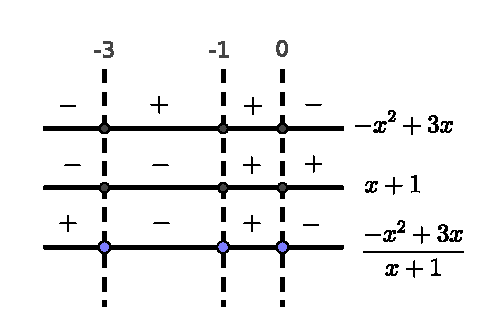
\includegraphics[width=8cm]{Capitulos/Figuras/sinais.pdf}
 \end{figure}

 Logo pelo jogo de sinais da figura acima, e considerando que a equação não pode ser calculada em $x= -1$, pois este número real zera o denominador, obtemos
 \[S= [-3, -1) \cup [0, +\infty)\]
 como conjunto solução desta inequação.

 \end{exem}


 \section{Equações com módulo}% (fazendo)}

   \vskip0.3cm
 \colorbox{azul}{
 \begin{minipage}{0.9\linewidth}
 \begin{center}
  As equações modulares são equações que apresentam expressões algébricas dentro de um módulo.
 \end{center}
 \end{minipage}}
 \vskip0.3cm

 Antes de começarmos a ver exemplos destas equações lembremos que para um número real $x$ qualquer:

 \[
\abs{x}= \begin{cases}
      -x, \ \ \text{se} \ \ x<0 \\
      x, \ \ \text{se} \ \ x \geq 0 \ .
     \end{cases}
\]

Além disso o módulo de um número real possui algumas propriedades listadas na \autoref{prop.modulo} que serão necessárias para a resolução de equações modulares.

Vejamos então alguns exemplos de equações modulares resolvidas.

\begin{exem} Equações com módulo:
 \begin{enumerate}
  \item Suponha que $a> 0$. Resolva a equação $\abs{x}= a$

  Pela definição de módulo temos:
  \[
  \begin{cases}
      -x= a, \ \ \text{se} \ \ x<0 \\
      x= a, \ \ \text{se } \ \ x \geq 0 \ .
     \end{cases}
     \Rightarrow
     \begin{cases}
      x= -a, \ \ \text{se} \ \ x<0 \\
      x= a, \ \ \text{se } \ \ x \geq 0 \ .
     \end{cases}
  \] 
 Portanto o conjunto solução desta equação é $S= \left\{-a, a \right\}$.
 
  \item Caso particular: $\abs{x}= 10$

  Pela definição de módulo temos:
  \[
  \begin{cases}
      -x= 10, \ \ \text{se} \ \ x<0 \\
      x= 10, \ \ \text{se } \ \ x \geq 0 \ .
     \end{cases}
     \Rightarrow
     \begin{cases}
      x= -10, \ \ \text{se} \ \ x<0 \\
      x= 10, \ \ \text{se } \ \ x \geq 0 \ .
     \end{cases}
  \]
 Portanto o conjunto solução desta equação é $S= \left\{-10, 10 \right\}$.

 \item $\abs{2x-2}= 10$

  Pela definição de módulo temos:
  \[
  \begin{cases}
      -(2x-2)= 10, \ \ \text{se} \ \ (2x-2)<0 \\
      2x-2= 10, \ \ \text{se } \ \ (2x-2) \geq 0
     \end{cases}
     \Rightarrow
     \begin{cases}
      -2x + 2= 10, \ \ \text{se} \ \ x< 1 \\
      2x - 2= 10, \ \ \text{se } \ \ x \geq 1
     \end{cases}
     \]
     \[
     \Rightarrow
     \begin{cases}
      -2x= 8, \ \ \text{se} \ \ x< 1 \\
       2x= 12, \ \ \text{se } \ \ x \geq 1
     \end{cases}
     \Rightarrow
     \begin{cases}
      x= -4, \ \ \text{se} \ \ x< 1 \\
      x= 6, \ \ \text{se } \ \ x \geq 1 \ .
     \end{cases}
  \]
  Portanto o conjunto solução desta equação é $S= \left\{-4, 6 \right\}$.  

  \item $\abs{2x^2 - 72}= 26$

  Novamente aplicando a definição de módulo temos
    \[
    \begin{cases}
      -(2x^2-72)= 26, \ \ \text{se} \ \ (2x^2-72)<0 \\
      2x^2- 72= 26, \ \ \text{se } \ \ (2x^2-72) \geq 0
     \end{cases}
     \]

     Como $2x^2- 72= 0 \Leftrightarrow 2x^2= 72 \Leftrightarrow x^2= 36 \Leftrightarrow \abs{x}= 6$ e a equação do 2º grau $2x^2- 72= 0$ tem $a> 0$, fazendo o estudo de sinal desta equação obtemos os três seguintes casos:
     \[
     \begin{cases}
      2x^2- 72 \geq 0, \ \ \text{se} \ \ x \leq -6 \\
      2x^2- 72 < 0, \ \ \text{se} \ \ -6 < x < 6 \\
      2x^2- 72 \geq 0, \ \ \text{se} \ \ x \geq 6 \\
     \end{cases}
     \]
     Com isso temos que a equação inicial deve ser dividida nos seguintes casos:
     \[
     \Rightarrow
      \begin{cases}
       2x^2- 72= 26, \ \ \text{se } \ \ x \leq -6 \\
      -(2x^2-72)= 26, \ \ \text{se} \ \ -6 < x < 6\\
       2x^2- 72= 26, \ \ \text{se } \ \ x \geq 6 \\
     \end{cases}
     \]
     temos portanto duas equações para resolver, façamos elas separadamente:
     \[2x^2- 72= 26 \Leftrightarrow 2x^2= 98 \Leftrightarrow x^2= 49 \Leftrightarrow x= \pm 7\]
     note que $-7 < -6$ e $7 > 6$ logo $x=-7$ e $x=7$ são soluções desta equação, agora vejamos o outro caso,
\begin{align*}
-(2x^2-72)= 26
& \Leftrightarrow -2x^2 + 72= 26 \\
& \Leftrightarrow -2x^2= -46 \\
& \Leftrightarrow x^2= 23 \\
& \Leftrightarrow x= \pm \sqrt{23} \approx \pm 4,78
\end{align*}

note que $-6< -\sqrt{23} < \sqrt{23} < 6$, logo $x=-\sqrt{23}$ e $x=\sqrt{23}$ são soluções desta equação. Portanto o conjunto solução da nossa é equação modular é:
     \[S= \{-7, -\sqrt{23}, \sqrt{23}, 7\} \ .\]

     \item \colorbox{yellow}{Atenção!} $\abs{x-4}=-2$

     Pela definição de módulo temos:
     \[
    \begin{cases}
      -(x-4)= -2, \ \ \text{se} \ \ (x-4) < 0 \\
        x-4 = -2, \ \ \text{se } \ \ (x-4) \geq 0
     \end{cases}
     \Rightarrow
     \begin{cases}
      -x+4= -2, \ \ \text{se} \ \ x < 4 \\
       x-4= -2, \ \ \text{se } \ \ x \geq 4
     \end{cases}
     \]
     \[
     \begin{cases}
      -x= -2-4, \ \ \text{se} \ \ x < 4 \\
       x= -2+4, \ \ \text{se } \ \ x \geq 4
     \end{cases}
     \Rightarrow
     \begin{cases}
      x= 6, \ \ \text{se} \ \ x < 4 \\
      x= 2, \ \ \text{se } \ \ x \geq 4
     \end{cases}
     \]
 Observe que em nenhum dos dois casos o $x$ encontrado pertence ao intervalo onde a solução deveria estar, pois $6$ não é menor que $4$ e $2$ não é maior ou igual a $4$, além disso,
 \[x=6 \Rightarrow \abs{6-4}= \abs{2}= 2 \neq -2\]
 \[x=2 \Rightarrow \abs{2-4}= \abs{-2}= 2 \neq -2\]
 logo esta equação NÃO tem solução!

 Mas isso já era de se esperar, pois lembra que $\abs{x}\geq 0$ para qualquer $x \in \R$, por propriedade do módulo, logo $\abs{x-4} \geq 0$ como $-2< 0$ então não existe $x \in \R$ tal que $\abs{x-4}= -2$. Portanto, já sabíamos pela propriedade de módulo que esta equação não tinha solução.

\end{enumerate}
\end{exem}

 Vamos agora, sistematizar o que acabamos de ver nos exemplos acima de forma a facilitar a aplicação desta teoria na resolução de equações modulares gerais. Para tal consideremos uma equação modular na forma geral
 \[\abs{A}= B\]
 em que $A$ e $B$ são expressões algébricas. Pela definição de módulo temos que
 \[ \abs{A}= \begin{cases}
          -A, \ \text{se} \ \ A < 0 \\
           A, \ \text{se} \ \ A \geq 0
         \end{cases}
 \]
 logo as soluções da equação modular devem satisfazer
 \[A= B \ \ \ \text{ou} \ \ \ -A= B \ .\]
 Além disso, lembremos que por propriedade de módulo $\abs{A}\geq 0$, então para ser uma solução da equação a variável $x$ deve também satisfazer esta propriedade. Mas como vimos no contra-exemplo acima nem toda variável satifaz
 \[(A= B \ \ \ \text{ou} \ \ \ -A= B) \ \ \ \text{e} \ \ \ (\abs{A}\geq 0) \ . \]
 Note que, como nossa equação é $\abs{A}= B$, logo garantir $\abs{A}\geq 0$ é equivalente a garantir $B \geq 0$, donde obtemos que as equações com $B < 0$ não possuem solução.

 Resumindo temos que,

  \vskip0.3cm
 \colorbox{rosa}{
 \begin{minipage}{0.9\linewidth}
 \begin{center}
   uma variável $x$ é solução da equação modular $\abs{A}= B$ se ela satisfizer:
 \[(A= B \ \ \ \text{ou} \ \ \ -A= B) \ \ \ \text{e} \ \ \ (B \geq 0) \ . \]
 \end{center}
 \end{minipage}}
 \vskip0.3cm

 Vejamos mais alguns exemplos resolvidos de equações com módulo.

 \begin{exem}
    $\abs{x-2} + \abs{x+4}= 10$

   Antes de começarmos a pensar em como resolver esta equação modular observe que $B= 10 \geq 0$, então uma das condições necessárias para se obter uma solução para a equação já está satisfeita, agora basta analisar os casos $A= B$ e $-A= B$.

   Para fazer esta segunda etapa da solução lembre-se que no exemplo \autoref{eqmodulo} após simplificarmos a expressão $\abs{x-2} + \abs{x+4}$, considerando os casos $A< 0$, $A= 0$ e $A> 0$ e obtemos:
   \[ \abs{x-2} + \abs{x+4} = \begin{cases}
      -2x-2, \ \ \text{se} \ \ x < -4 \\
      6, \ \ \text{se } \ \ -4 \leq x < 2 \\
      2x + 2, \ \ \text{se} \ \ x \geq 2 \ .
     \end{cases}
  \]
 Agora para resolver esta equação modular vamos usar esta simplificação da expressão. Assim note que temos três casos para analisar, façamos eles separadamente.

 \textbf{Caso 1:} $x < -4$

 Neste caso, $\abs{x-2} + \abs{x+4}= -2x-2$, com isso temos que nossa equação se torna:
 \[-2x-2= 10 \Rightarrow -2x= 12 \Rightarrow x= -6\]
 como $x= -6$ satisfaz a inequação $x< -4$, ele é uma solução.

 \textbf{Caso 2:} $-4 \leq x < 2$

 Neste caso, $\abs{x-2} + \abs{x+4}= 6$, com isso temos que nossa equação se torna:
 \[6= 10\]
 o que é impossível, donde concluímos que neste intervalo a equação não tem solução.

 \textbf{Caso 3:} $x \geq 2 $

 Neste caso, $\abs{x-2} + \abs{x+4}= 2x + 2$, com isso temos que nossa equação se torna:
 \[2x + 2= 10 \Rightarrow 2x= 8 \Rightarrow x= 4\]
 como $x= 4$ satisfaz a inequação $x \geq 2$, ele é uma solução da equação.

 Portanto obtemos $S=\{-6, 4\}$ como conjunto solução da equação modular
\[\abs{x-2} + \abs{x+4}= 10 \ .\]

 \end{exem}


 \section{Inequações modulares}% (fazer)}

 Nesta seção iremos usar as propriedades da ordem do conjunto dos números reais e também as propriedades de módulo de um número real. Neste momento já supomos que o leitor está bem familiarizado com as estas propriedades, mas na dúvida você pode consultar as propriedades que estão listadas nas \autoref{prop.ordem} e \autoref{prop.modulo}.
 
 \begin{exem} Vejamos agora alguns exemplos de inequações modulares.
  \begin{enumerate}
   \item Suponha que $a> 0$. Resolva a inequação $\abs{x} < a$.
   \[\abs{x} < a \Leftrightarrow \abs{x}^2 < a^2 \Leftrightarrow x^2 < a^2\]
   mas,
   \[x^2 < a^2 \Leftrightarrow x^2 - a^2 < 0 \Leftrightarrow (x-a)(x+a) < 0 \ .\]
   Vamos então analisar quando $(x-a)(x+a) < 0$. Lembremos que produto de dois números é negativo quando um deles for negativo e o outro positivo, com isso a inequação $(x-a)(x+a) < 0$ é satisfeita em duas situações:\\
   Caso 1: $x-a<0$ e $x+a>0$
   \[x-a<0 \Rightarrow x< a\]
   e 
   \[x+a>0 \Rightarrow x>-a \Rightarrow -a< x\]
  Fazendo a interseção dos conjuntos $A_1= \left\{ x \in \R \mid x<a \right\}$ e $B_1= \left\{ x \in \R \mid -a<x \right\}$, obtemos $A_1 \cap B_1= \left\{ x \in \R \mid -a< x <a \right\}$. O conjunto $A_1 \cap B_1$ é o conjunto solução da inequação neste caso.

   
   Caso 2: $x-a>0$ e $x+a<0$
   \[x-a> 0 \Rightarrow x> a\]
   e
   \[x+a< 0 \Rightarrow x<-a\]
   Fazendo a interseção dos conjuntos $A_2= \left\{ x \in \R \mid x> a \right\}$ e $B_2= \left\{ x \in \R \mid x<-a \right\}$, obtemos $A_2 \cap B_2= \emptyset$. Portanto neste caso a inequação não possui solução.
  
  Portanto $\abs{x} < a \Leftrightarrow -a< x <a$.
   
   \item Caso particular: $\abs{x} \leq 5$
   \[\abs{x} \leq 5 \Leftrightarrow -5 \leq x \leq 5\]
   logo, o conjunto solução desta inequação é:
   \[S= [-5, 5] \ . \]

   \item Suponha que $a> 0$. Resolva a inequação $\abs{x} > a$.
   \[\abs{x} > a \Leftrightarrow \abs{x}^2 > a^2 \Leftrightarrow x^2 > a^2\]
   mas,
   \[x^2 > a^2 \Leftrightarrow x^2 - a^2 > 0 \Leftrightarrow (x-a)(x+a) > 0 \ .\]
   Vamos então analisar quando $(x-a)(x+a) > 0$. Lembremos que produto de dois números é positivo quando eles tem o mesmo sinal, com isso a inequação $(x-a)(x+a) > 0$ é satisfeita em duas situações:\\
   Caso 1: $x-a< 0$ e $x+a< 0$
   \[x-a< 0 \Rightarrow x< a\]
   e 
   \[x+a< 0 \Rightarrow x< -a \ .\]
  Fazendo a interseção dos conjuntos $A_1= \left\{ x \in \R \mid x<a \right\}$ e $B_1= \left\{ x \in \R \mid x< -a \right\}$, obtemos $A_1 \cap B_1= \left\{ x \in \R \mid x< -a \right\}$. O conjunto $A_1 \cap B_1$ é o conjunto solução da inequação neste caso.
 
   
   Caso 2: $x-a> 0$ e $x+a> 0$
   \[x-a> 0 \Rightarrow x> a\]
   e
   \[x+a> 0 \Rightarrow x> -a \]
   Fazendo a interseção dos conjuntos $A_2= \left\{ x \in \R \mid x> a \right\}$ e $B_2= \left\{ x \in \R \mid x> -a \right\}$, obtemos $A_2 \cap B_2= \left\{ x \in \R \mid x> a \right\}$. O conjunto $A_2 \cap B_2$ é o conjunto solução da inequação neste caso.
   
   Agora fazendo $S= (A_1 \cap B_1) \cup (A_2 \cap B_2)$ obtemos que $S= \left\{ x \in \R \mid x<-a \text{ ou } x> a \right\}$ é o conjunto solução da inequação $\abs{x} > a$.
  
  Portanto $\abs{x} > a \Leftrightarrow x<-a \text{ ou } x> a$.
   
   \item Caso particular: $\abs{x} \geq 5$
   \[\abs{x} \geq 5 \Leftrightarrow x \leq -5 \ \ \text{ ou } \ \ x \geq 5\]
   logo, o conjunto solução desta inequação é:
   \[S= (-\infty, -5] \cup [5, \infty) \ . \]

  \end{enumerate}

 \end{exem}


% \section{Equações com raízes (fazer)}

% \section{Inequações com raízes (fazer)}
